\documentclass[10pt]{article}
\usepackage[utf8]{inputenc}
\usepackage[T1]{fontenc}
\usepackage{a4wide}
\usepackage{float}
\usepackage[version=4]{mhchem}
\usepackage{stmaryrd}
\usepackage{multicol}
\usepackage[export]{adjustbox}
\usepackage{hyperref}
\usepackage{dirtree}
\graphicspath{ {./images/} }
\hypersetup{colorlinks=true, linkcolor=blue, filecolor=magenta, urlcolor=cyan,}
\urlstyle{same}
\setlength\columnsep{25pt}

\usepackage{array}
\newcolumntype{P}[1]{>{\centering\arraybackslash}p{#1}}


\title{WET - Water Efficiency Tool }

\iffalse
\author{
  Bessis, Hugoo\\
  ESILV\\
  Paris, France\\
  hugob6@orange.fr
  \and
  Saouab, Oumniya\\
  Al Akhawayn University\\
  Casablanca, Morocco\\
  oumniyasaouab@gmail.com
  \and
  Utama, Takara Izzah\\
  Hanyang University\\
  Seoul, South Korea\\
  takaraizzahutama@gmail.com
  \and
  van der Heide, Niklas\\
  ZHAW - School of Applied Sciences\\
  Winterthur, Switzerland\\
  niklasvdh@gmx.ch
}
\fi

\begin{document}
\maketitle

\begin{table}[H]
  \centering
  \begin{tabular}{P{5.5cm}P{1cm}P{5.5cm}}
    Bessis, Hugoo & & Saouab, Oumniya \\
    ESILV & & Al Akhawayn University \\
    Paris, France & & Casablanca, Morocco \\
    hugob6@orange.fr & & oumniyasaouab@gmail.com \\
     & &  \\
     & &  \\
    Utama, Takara Izzah & & van der Heide, Niklas \\
    Hanyang University & & ZHAW - School of Applied Sciences \\
    Seoul, South Korea & & Winterthur, Switzerland \\
    takaraizzahutama@gmail.com & & niklasvdh@gmx.ch \\
  \end{tabular}
\end{table}

\vspace{1cm}

\begin{abstract}
House owners that have tight schedules or have a busy lifestyle tend to forget to monitor their houses properly. For example, they forget to close a water tap after using it. To check every water tap is closed properly or to make sure you are not using your water recklessly consumes time and requires a family member to be at the house. Therefore, our team is trying to develop an application (app) that monitors the water consumption in real time. The app not only provides real time monitoring but also provides users with consumption history, consumption limits, leakage detection, and consumption forecast. The primary goal of this app is to enable a user to monitor the water usage through a mobile application. This would help people structure their water usage more efficiently and change habits of consumption.
\end{abstract}

\clearpage

\begin{multicols*}{2}

\section{Role Assignments}

\begin{itemize}
  \item {User} \\
  Users are people owning a home equipped appliances that include the necessary sensors and internet access. The User role should help the team better analyze what features are actually useful and to judge the current user experience.\\
  This role will be filled by Oumniya Saouab.
  \item {Customer} \\
  A home appliance company that wants to give their users the possibility to manage their appliances by using WET would be our customer. This role will help in creating a product that could actually be sold and generate profit.\\
  This role will be filled by Takara Utama.
  \item {Software Developer} \\
  The software developer thinks, designs, and realizes the software in general. Their goal is to implement all the requirements.\\
  This role will be filled by Niklas van der Heide.
  \item {Development Manager} \\
  Development Manager is the person in charge of supervising their team's work throughout the app's development. They should have a good overview over what features are being worked on and by whom.\\
  This role will be filled by Hugo Bessis.
\end{itemize}

\iffalse
\begin{table}[!ht]
\centering
\begin{tabular}{| p{0.01\linewidth} | p{0.1\linewidth} | p{0.1\linewidth} |}
\hline
Role & Project Member & Description \\
\hline
User & Oumniya & Users are people owning a home equipped appliances that include the necessary sensors and internet access. The User role should help the team better analyze what features are actually useful and to judge the current user experience. \\
\hline
Customer & Takara & A home appliance company that wants to give their users the possibility to manage their appliances by using WET would be our customer. This role will help in creating a product that could actually be sold and generate profit. \\
\hline
Software Developer & Niklas & The software developer thinks, designs, and realizes the software in general. Their goal is to implement all the requirements. \\
\hline
Development Manager & Hugo & Developer Manager is the person in charge of supervising their team's work throughout the app's development. They should have a good overview over what features are being worked on and whom. by \\
\hline
\end{tabular}
\end{table}
\fi

\section{Introduction}
Managing water consumption is vital for life preservation. Better knowing one's water consumption at home can have a great impact on water saving. Even families could change habits of consumption. Reports have warned of an impending global water crisis due to surging population growth, climate change, reckless consumption, and chronic waste. We hope to help people to use water more responsibly to help stop the global water crisis. While trying to do some research on similar apps, we were not able to find that many existing projects. Thus, we are motivated to provide a solution to this problem.

Our application provides some features that help the user to monitor their water consumption in real time, let users know their consumption history based on day, weeks, etc. Also, the app let users limit their usage so that they could save water and money and even gave them the consumption forecast, so that they could change their habit if they are using water recklessly. As a result, we hope that this application will help the problem of the water crisis that is currently happening in the world right now.


\section{Problem Statement}
The Water Efficiency Tool is a project hoping to help people monitor and manage their water consumption. In this form we envision the application user to actively monitor their water consumption, and if there is any water running for an unusual duration the app will give you a notification about it, and you can remotely close the central water supply to make it stop. In other words, the Water Efficiency Tool is a project that aims to assist people in tracking and controlling their water usage. In its current form, the application allows users to actively monitor their water usage. If any water is left running for a length of time that is unusual, the app will notify the user and allow them to remotely shut off the main water supply to stop it.

Saving water or using water with responsibility is something that has been going on for years, but to actually do it or to encourage people to do so is a hard thing to do. Because excessive water use can go unnoticed. Water bills are relatively cheaper than other utilities. Compared to other problems, benefits of reducing water consumption are not necessarily felt by the individual. And many people don't believe that individual actions can make much of a difference compared to the amount of water lost through leakages. As a result, some other parts of the world are having a water crisis and shortage.

\clearpage

\section{Related Software}

\begin{enumerate}

  \item {Dropcountrer ${ }^{[1]}$}
  
  This app lets you know how much water you are using and sets benchmarks for conserving with this new web and mobile app that tracks water usage in real time and sends a usage warning to your device or smartphone if you're nearing overuse. In addition to that, the app connects to local utility companies and water districts to help users track water consumption. Adding to the daily tracking feature, the app sends users alerts on rebates and other preventative water-waste actions. App downloaders can also take advantage of the utility poke, which locates your water district and contacts them requesting user data.

  \item {Drip Detective ${ }^{[2]}$}
  
  Drip Detective is an application tells you how much water and money is going down the drain by timing leaks or measuring volume, then calculating the cost of your water leak by day, week, month, and year, in other words, by timing leaks or measuring volume, the application Drip Detective estimates how much water and money are being wasted. It then calculates the cost of your water leak by day, week, month, and year.

  \item {Klima ${ }^{[3]}$}
  
  Klima is a climate app that allows you to offset your emissions, reduce your carbon footprint and multiply your carbon impact. To do that, the app calculates a member's annual carbon footprint by asking them 9-10 lifestyle questions, including how they eat, whether they have a car, or how often they take a flight. These factors are used to calculate the user's estimated carbon footprint. It is not exatcly what our app will look like, but the purpose of the app is quite similar, which is trying to help the world.

  \item {Kill-Ur-Watts ${ }^{[4]}$}
  
  It is an application that permits residential customers to view, track, and manage their residential electricity use over time. This application utilizes common industry-based concepts and third-party data to empower residential users to make informed decisions on energy reduction strategies and implement common-sense energy efficiency improvements. Kill-Ur-Watts allows users to view hourly, daily, and monthly home energy consumption profiles and use social media outlets to challenge other users to reduce energy consumption. These 2 features are quite the same features that we are going to have on our application, which are to track our water consumption as well as our gamification, where we could share our achievement that we get for using water with responsibility to our social media.

  \item {Nest ${ }^{[5]}$}
  
  Nest is an app that lets you control the thermostat, alarm system, and camera. The approach of this app is quite similar to our app, which is trying to control the unused water. For example, from an unclosed water tap.

\end{enumerate}

\clearpage

\section{Requirements}

Before starting with any development it is important to make it clear what the application should actially do. To make sure everyone is on the same page and to create a concrete plan, the following requirements for our app have been defined. We allowed ourselves to change any requirement if necessary. A requirement change should always be discussed in the team to avoid confusion.

\begin{enumerate}
  \item {User Registration}
  
  A new user should be able to register themselves on the app. To do that they need to provide the following information:

  \begin{itemize}
    \item Full Name
  
    \item Address
  
    \item Country
  
    \item Phone Number
  
    \item Email
  
    \item Password
  
  \end{itemize}

  The user's email or phone number should be verified to ensure their authenticity. The set email or phone number together with the given password will be used to authenticate and login the user.

  \item {User Login}\\
  After a user has been successfully registered they should be able to log in to the app with their email or phone number together with the correct password. Only when logged in should the user be able to access, manage or change their home's information.

  \item {Device Registration} \\
  Home appliances that include the necessary wifi capability as well as the sensors to capture the information relevant to the system should be able to be registered in the app. To add a new device, the user must be logged in and connected to the same network as the appliance to be added.
  
  \item {Modifying unit and language settings} \\
  The user should be able to modify the unit settings. For the volume of water, the user can change the metric by liter, cubic meter or gallons. The user can also choose which currency to display, and the app language.
  \item {Real Time Monitoring} \\
  A user should be able to monitor their water consumption in real time. The App should be able to display what devices are currently using up water and at what rate. This would give the user the comfort of knowing that there is no unexpected or wasteful water usage.
  \item {Consumption History} \\
  The App should display and visualize the homes past water usage over different time periods:

  \begin{itemize}
    \item 1 day
  
    \item 1 Week
  
    \item 1 Month
  
    \item 1 Year
  
    \item All
  
  \end{itemize}

  The user should be presented with the hard numbers as well as visual representations in the form of charts and graphs.

  \item {Consumption Limits}\\
  To help the user save water and money, they should be able to set a limit for the time frames:

  \begin{itemize}
    \item daily limit
  
    \item weekly limit
  
    \item monthly limit
  
  \end{itemize}
  
  They should be able to set the limits based on the amount of water or cost.
  
  Once a limit is reached, the user should be notified of that.


  \item {Leakage Detection} \\
  The Application should alert the user if an appliance is using up water for an unusual duration or at an irregular rate.
  
  \item {Remote Control} \\
  When leaving for a longer duration of time, the user should be able to remotely close the central water supply to not use any water. If appliances can be separately disabled, the user should be able to disable them separately. \\
  If any water is used despite the appliance or the central water supply is dissabled, the user should be notified.

  \item {Consumption Forecast} \\
  This feature helps the user to predict its water consumption for the next week. When the user clicks on this, they should be able to see the volume of water they will most likely consume the next week based on the previous week's water consumption.

  The user can also click on the cost prediction button that will display the predicting cost of their water consumption for the next week based on their previous week's water consumption.

  The user can also select the time frame of the prediction and get either a week, a month or a year prediction.

  This feature will help the user to adapt its consumption to prevent over consumption usage of water.

  \item {Gamification} \\
  When the user is clicking on the badges button, it will display all the badges and achievements they made using the apps. These can be earned by using the app through the time. The badges and achievements will reward the user for consuming water responsibly, according to government laws and international recommendations (COP21, GIEC, etc.). The user will be able to share their achievements and badges on social media such as Twitter, Instagram and Meta.

\end{enumerate}

\clearpage

\section{Tools and Environment}

\begin{enumerate}
  \item {Operating System} \\
  We are going to develop applications using mac OS and Windows as our main development platforms. Windows is a good choice for programming since it provides many useful programs. And the whole Windows development stack is amazing. MacOS is also a good option for someone that works on a back-end server because it's based on Unix and runs nearly all Linux software.
  
  \item {Programming Languages} \\
  The main part of our code base is the App front end. For this we have decided to use $Flutter$ and $Dart$ to enable cross platform compatability. For the backend API that manages the data transfer between the database and the app $Node.js$ will be used. $Node.js$ is a good solution since there already exist many packages to help acheive the required functionality.
  
  \item {Development Environment}
  \begin{itemize}
    \item {Visual Studio Code} \\
    Our project consists of many different files in different languages and environments. The versatile plug in system that Visual Studio Code provides helps out greatly with this problem. There is an appropriate extension for each file type to enable code highlighting. Visual Studio Code also provides basic IDE features like compilers debuggers, and code completions.
    \item {Android Studio} \\
    Android Studio provides emulators for Android based phones. The written front end code can be quiqly tested by running an emulator that constantly runs the most recent code. Android Studio can also be used as an IDE for $Flutter$ and $Dart$ development.
    \item {GitHub} \\
    GitHub is free online service to host and manage Git repositories. With GitHub we can manage the code with propper version controll. GitHub also allows for pull request wich allows the more experianced team members to review and comment on the other members code before merging it into the main code base.
    \item {Postman} \\
    Postman is a tool to test APIs. Requests of all types can be created and reused at a later time. This tool is a big time saver when working on an API wich is why we decided to use it.
  \end{itemize}

  \item {Services} \\
  To allow our Application to function, different services are required. Here is a list of the ones we employ.
  \begin{itemize}
    \item {Firebase} \\
    Firebase is used for its simple and easy to use user managements service. Users can be registered and authenticated.
    \item {MongoDB} \\
    A big part of the application is the data the different appliances provide. This data is stored in a $MongoDB$ database. $MongoDB$ is especially usefull since the data can be stored and directily retreived in $JSON$ format.
    \item {AWS} \\
    The MongoDB database is stored on a local AWS server. The management of that server is fully done by the $MongoDB$ online application.
  \end{itemize}

  \item {Software In Use}
  Other than the development tools mentioned above, some other software is used to help with development
  \begin{itemize}
    \item {MiKTeX} \\
    To work on this document, wich is written in LateX a way of rendering the written text to a PDF file. MiKTeX provides the feaetures to do this. It manages and automatically downloades the included libraries and plugins.
    \item {Umlet} \\
    Umlet is a useful tool to create simple UML diagrams. We used it to create the Use Case Diagram seen below.
    \item {diagrams.net} \\
    Formaly known as draw.io, doagrams is a useful tool for more dynamic diagrams and other ilustration. It was used to creat the applications architecture diagram.
    
  \end{itemize}
\end{enumerate}

\clearpage

\section{Specification}

\begin{enumerate}
  \item {User Login Page} \\
  When the user opens the app, he will get the login page. They can either create a new account by choosing the register option, or login if they already have an account. \\
  To log in, the user must fill in their mail address or phone number, and password. They can also check the "Remember me" mark to stay connected every time the app is closed and reopened. \\
  \begin{center}
    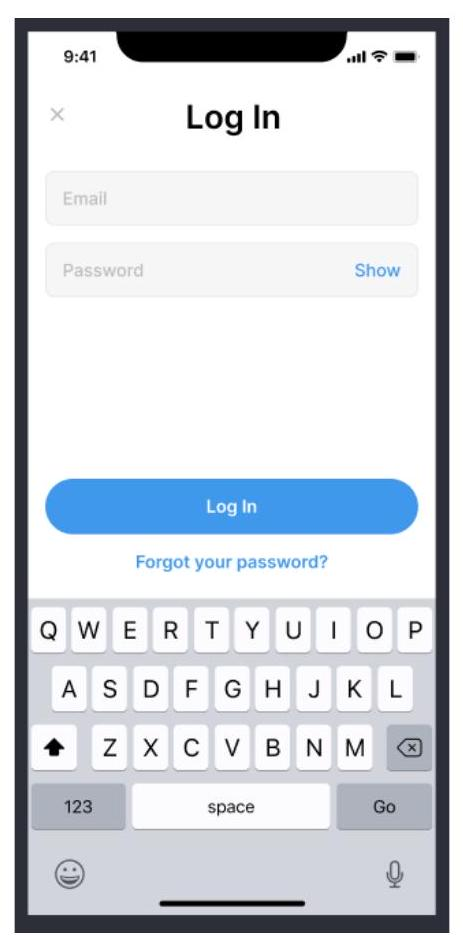
\includegraphics[max width=4cm]{login.jpg}
  \end{center}

  \item {User Registration Page} \\
  When choosing the register option on the login page, the user should be asked to fill in personal information such as:
  \begin{itemize}
    \item full name
    \item home address
    \item country of residence
    \item phone number
    \item email
    \item a password
  \end{itemize}
  They will receive a SMS and email confirmation to confirm the creation of their account.
  
  \begin{center}
    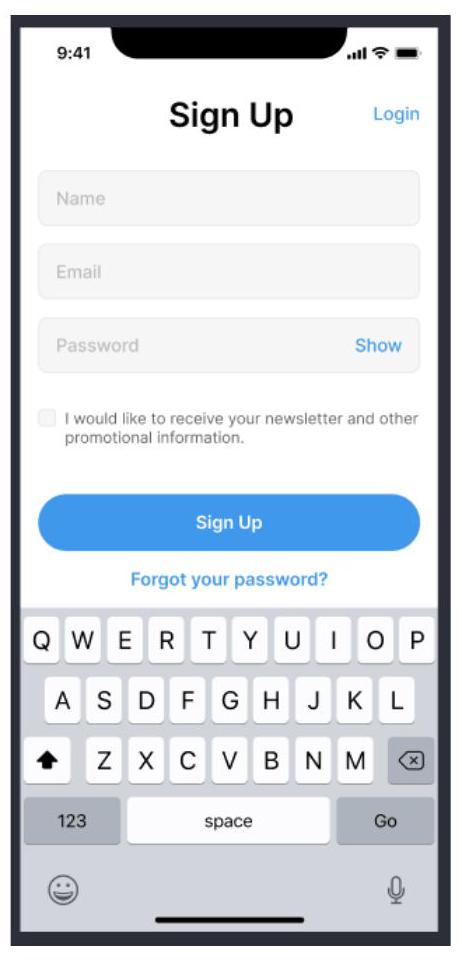
\includegraphics[max width=4cm]{signup.jpg}
  \end{center}

  \item {House Registration Page} \\
  After logging in for the first time or by choosing the "register devices" option on the profile settings page, the user will be asked to register their home appliance devices into the app.\\
  In order to do that, the user has to be connected to each appliance's personal Wi-Fi network. After the connection has been established the app will automatically find all the compatible devices connected. The user can manually change the name of the device to create a more enjoyable experience. We found that the technical name of most devices do not properly describe their function.

  \begin{center}
    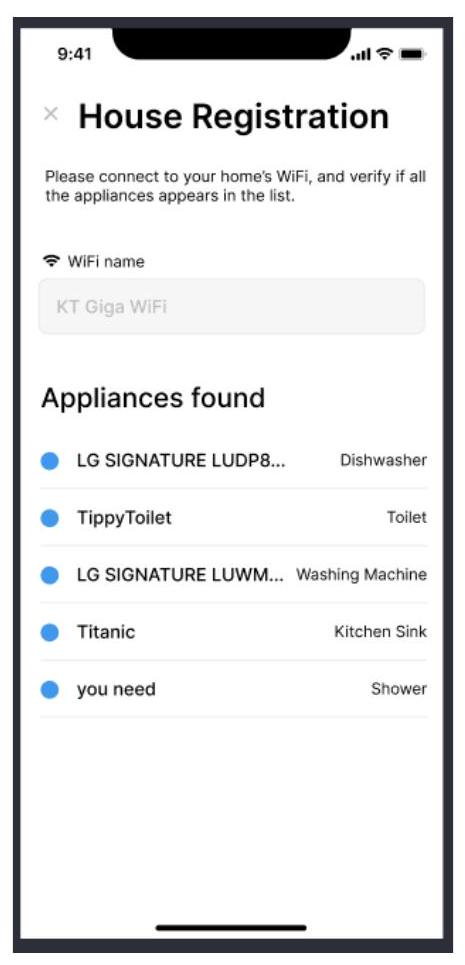
\includegraphics[max width=4cm]{houseregistration.jpg}
  \end{center}

  \item {Main Page} \\
  After finishing registering everything and or logining in, the user will be shown the main page. On this page, the app will display a statistical overview of the relevant happenings. This overview should include.

  \begin{itemize}
    \item That days water usag
    \item Appliance status
    \item Overview if daily, weekly or monthly usage goals have been failed or how far away from failing the user is.
  \end{itemize}
  
  The days water usage should be shown as a percentage of the set usage goal. A circle should be filled up with $100 \%$ filled representing $100 \%$ of the goal reached.
  
  \begin{center}
    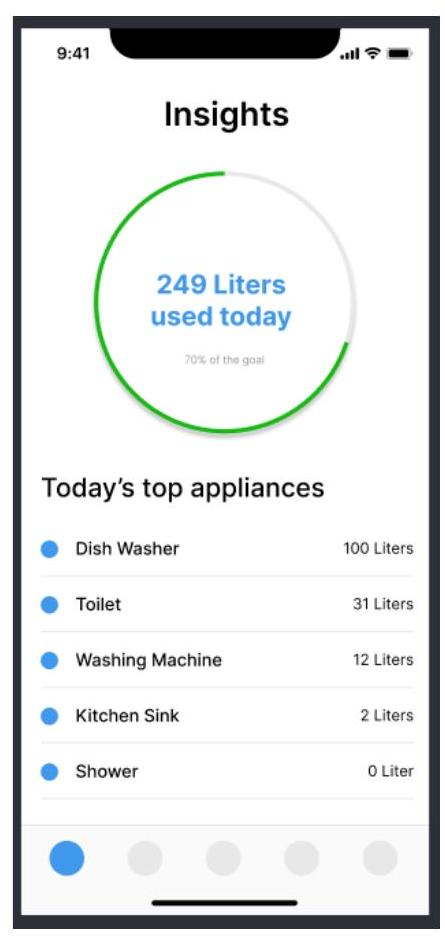
\includegraphics[max width=4cm]{mainpage-1.jpg}
  \end{center}

  Should the user's set goal be failed, the graph that displays the percentage of the goal reached should also reflect that.
  
  \begin{center}
    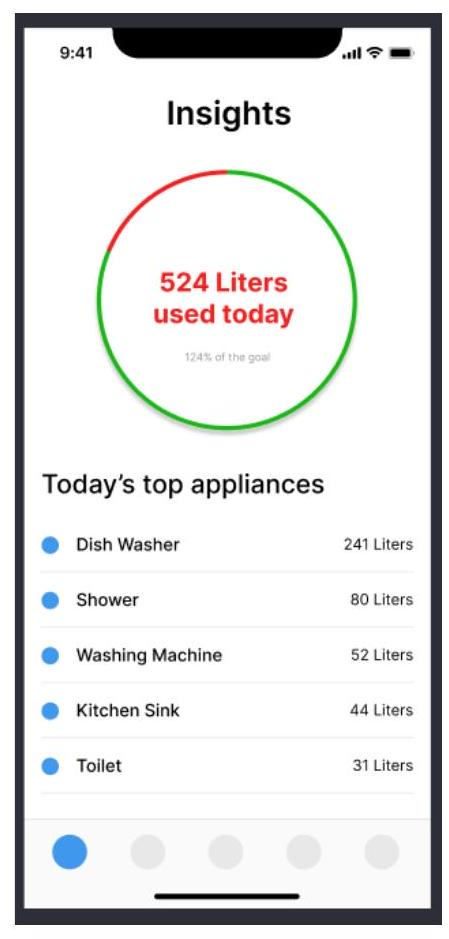
\includegraphics[max width=4cm]{mainpage-2.jpg}
  \end{center}

  \item {Consumption History and Forecast Page} \\
  In the Consumption History and Forecast Page, the user will see a line chart showing water consumption over a selected time frame. The user can modify the time frame of the chart:

  \begin{itemize}
    \item current day
    \item current week
    \item current month
  \end{itemize}

  At the bottom of the page there is a list of all appliances. The user is able to click on each device to show the consumption of only the selected device over the selected time period.

  On the same page the current water consumption is extrapolated and an estimated consumption for the selected time period is calculated. Should the estimated water consumption be higher than the set consumption goal, the user is warned of that.

  In the list of all appliances at the bottom of the page the current status of each appliance is visible. If an appliance is currently running the status should be "active" if not, "inactive". For "active" devices their current rate of consumption is also noted in the form of liters per minute.

  All numbers are rounded to the first decimal.

  \begin{center}
    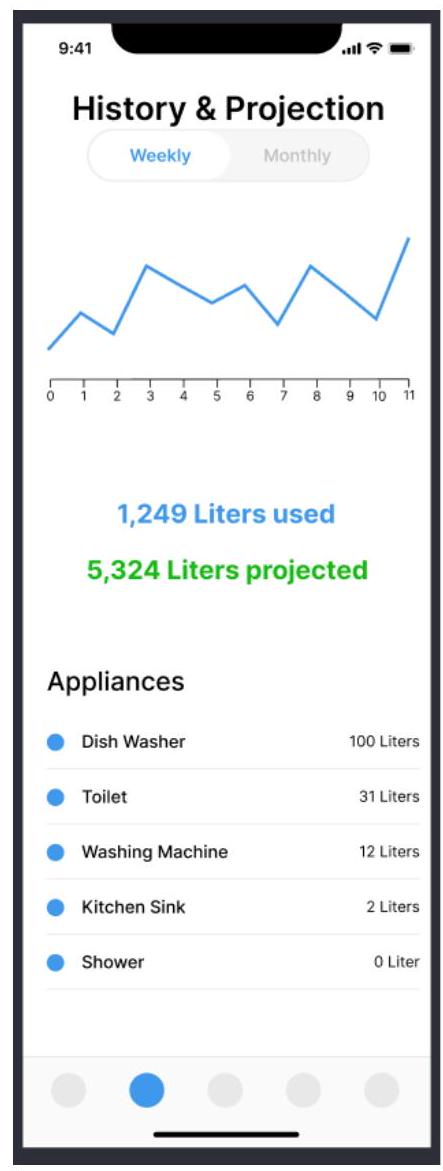
\includegraphics[max width=4cm]{historyandprojection.jpg}
  \end{center}

  \item {Holiday Mode Page} \\
  On the Holiday Mode Page the user is able to set their whole house to "holiday mode". If the home is in "holiday mode" the user is automatically notified if any water is used up at irregular amounts. On the same page, the idea of holiday mode is explained to the user.

  \begin{center}
    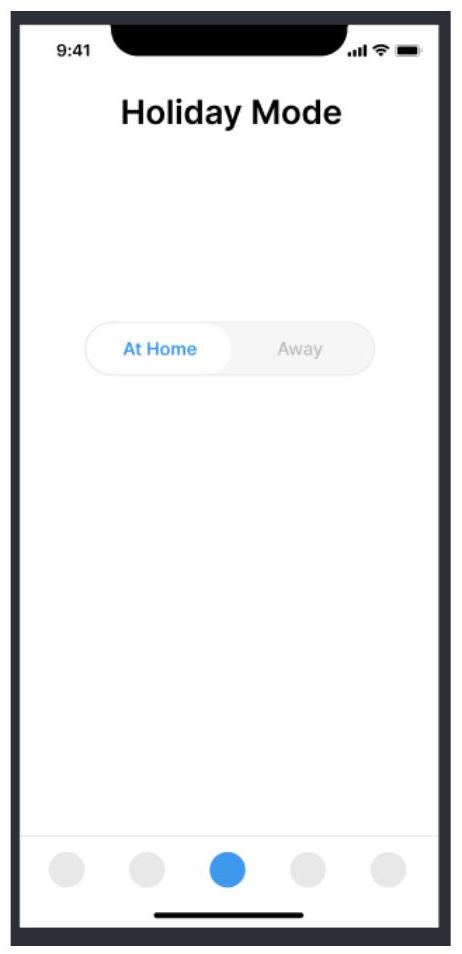
\includegraphics[max width=4cm]{holidaymode.jpg}
  \end{center}

  \item {Notifications Page} \\
  On the Notification Page the user is presented with all previous notifications. If a notification has not yet been seen by the user, it is marked as "unread".

  \begin{center}
    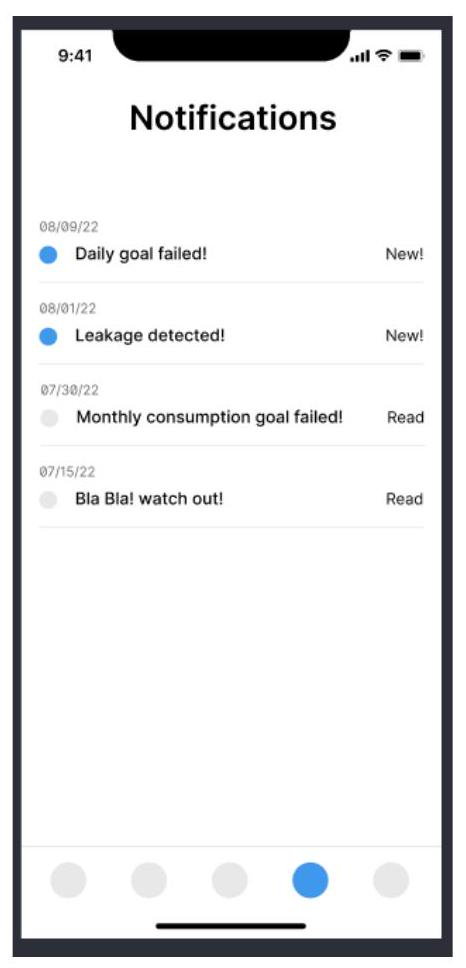
\includegraphics[max width=4cm]{notifications.jpg}
  \end{center}

  \item {Profile Settings Page} \\
  After registering a new account, the user will have to select some settings according to its country and metrics regulation, such as litter, cubic meter or gallons for the volume metric. They also have to choose the language they want to use as well as the currency such as US dollar, Euro, KRW, etc. for cost estimates.

  The Profile Settings Page also allows the user to set their consumption goal. This number is the amount of water to be consumed in a month. The unit is the one selected by the user and the number is an integer.

  The option to delete the users account can also be found a t the bottom of the Profile Settings Page.

  \begin{center}
    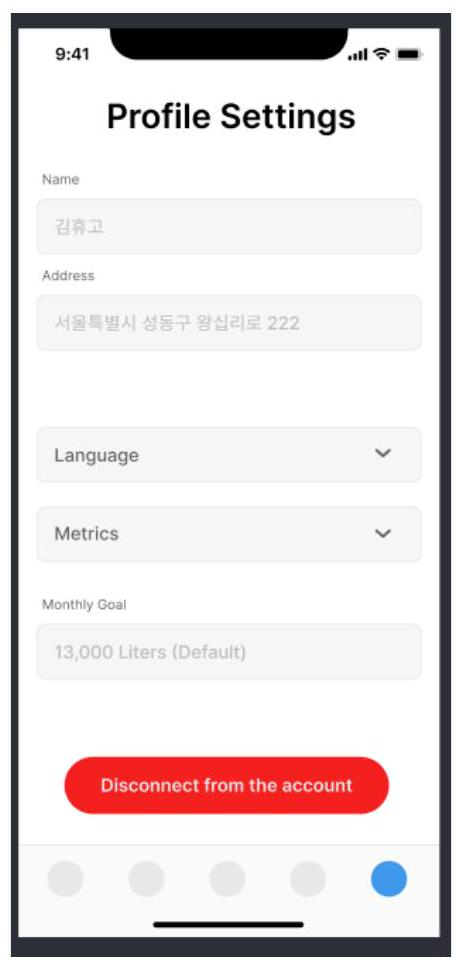
\includegraphics[max width=4cm]{profilesettings.jpg}
  \end{center}

  \item {Navigation Bar}
  On the bottom of the app, the user can click on different icons that are lined up side to side. Each icon takes the user to a page specified above.
  \begin{itemize}
    \item {Main Page}
    \item {Consumption History and Forecast Page}
    \item {Holiday Mode Page}
    \item {Profile Settings Page}
  \end{itemize}

\end{enumerate}

\clearpage

\section{Architecture Design}

\iffalse
\dirtree{%
  .1 /.
  .2 API.
  .3 models.
  .3 routes.
  .2 App Files.
  .2 Documentation.
  .3 Figma.
  .3 Latex.
}
\fi

\begin{enumerate}
  \item {System Architecture} \\
  The overall system Architecture of the WET infrastructure is quite simple.
  Users interract with the system through the app, which is installed on their mobile device. This mobile app represents the entire Front end.

  This app internaly calls the required back end services these services are comprised of the authentication service as well as a service that manages the data produced by the smart appliances.
  With the help of Firebase the app is able to connect directily to its authentication service without the need for any further backend infrastructure.
  The users data is stored in a $MongoDB$ database. To manage its access another facade interface in the form of a Node.js server was created. The Node.js server is manages requests and responses to and from the front end.

  This Architecture is what was used to create the MVP (minimum viable product). If the idea of WET would be developed into a fully fledged product the architecture would have to be reworked and extended.

  \begin{center}
    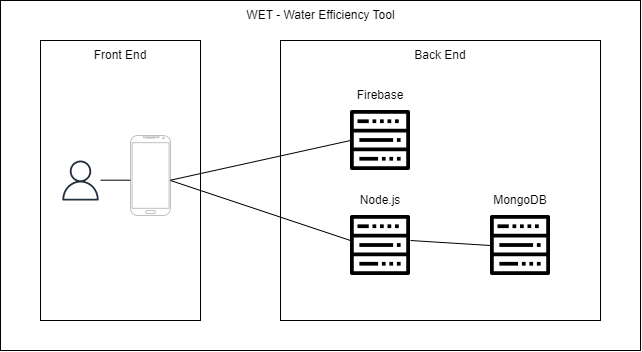
\includegraphics[max width=6cm]{uml/architecture}
  \end{center}
  
  \item {Directory Organisation} \\
  The code that is used to run our application as wellas its documentation is stored in vareous folders inside a GitHub repository.
  This the basic folder structure and a short description of what each folder is used for:

  \begin{center}
    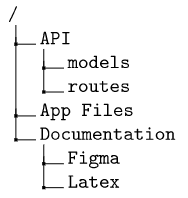
\includegraphics[max width=3cm]{repoTree}
  \end{center}

  \begin{itemize}
    \item {API} \\
    The API folder stores all code used to run the Node.js backend used to connect to the MongoDB storing the appliance data.
    \begin{itemize}
      \item {models} \\
      The folder contains all database models used to define the structure of the data stored inside the MongoDB.
      \item {routes} \\
      Inside the routes folders are the definitions of all the possible acces points to the API that can be used by the front end as well as appiances to send and receive data.
    \end{itemize}
    \item {App Files} \\
    The App Files folder defines the front of the application. It stores the code that is used to compile the mobile application as well as all other supporting scripts.
    \item {Documentation} \\
    An important part of any poject is its documentation. The documentation of our project is also stored inside the GitHub repository to allow collaboration.
    \begin{itemize}
      \item {Figma} \\
      The layout of the mobile application was first designed in Figma. This folder stores all those designs and related documentation.
      \item {Latex} \\
      This documentation is written in Latex. The raw Latex code used to generate the pdf document as well as all images that are included in it are stored inside this folder.
    \end{itemize}
  \end{itemize}

  \item {Module 1 (App)} \\
  The frontend is accting is the main interraction interface the users use to interract with the entire application. The mobile application allows the user to see the data genereated by their home smart appliances and all other functional requirements listed.
  All frontend code is located in the "./App Files" folder on the GitHub repository.
  \item {Module 2 (Server)} \\
  The backend server is used by the frontend mobile application to access the the data stored by the MongoDB database. It is also the access point used by the appliances to send their data to.
  All backend code is located in the "./API" folder on the GitHub repository.
\end{enumerate}

\clearpage

\section{Use Cases}

We compiled some of the most essential use cases of our application. These use cases should make it clear what is expected from the application and how a user would acheive the described task.
For a quick overview of the described use cases and how the user and other actors take part in them, see the following use case diagram.

\begin{center}
  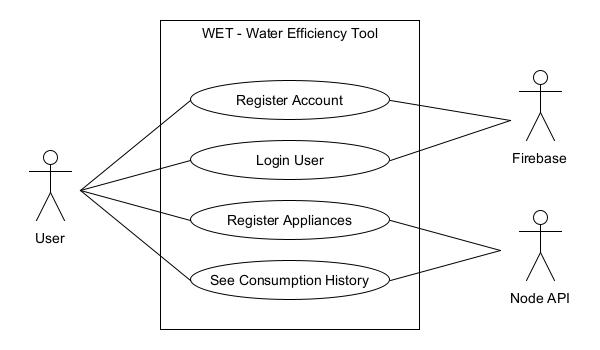
\includegraphics[max width=6cm]{uml/usecase_diagram}
\end{center}

\begin{itemize}
  \item {Register Account} \\
  Useres should be able to register a new account.
  
  After a user moves into a new home or downloades the WET app for the first time, they should be able to create a new account to allow them to register their devices and acces the generated data.
 
  Here are the steps taken by the user:
  \begin{enumerate}
    \item Open WET mobile app
    \item Click the "Register" button
    \item Enter user information
    \item Confirm information
    \item Confirm signup
  \end{enumerate}

  After registering a new account the user can log in and start using the application.
  
  \item {Login} \\
  Users should be able to log in to their account.

  Logging in with their account should allow the user acces to the data generated by their appliances. They should also be allowed to change user settings, add more appliances and delete their account.
  For a user to be able to log in to their account, they must have registered an account beforehand.
 
  Here are the steps taken by the user:
  \begin{enumerate}
    \item Open WET mobile app
    \item Enter user credentials and password
    \item Click the "Login" button
  \end{enumerate}

  After logging in the user can procede to use the application and its other features.

  \item {Register Applicance} \\
  Users should be able to register their appliances.

  For a user to be able to see their appliances data, these appliances have to be registered to their account. This way when requesting the generated data, the data from the corresponding users appliances can be returned.
  For a user to be able to register appliances, they must have registered an account beforehand.
  
  Here are the steps taken by the user:
  \begin{enumerate}
    \item Login (see use case "Login")
    \item Open settings table
    \item CLick the "Register Devices" button
    \item Connect to appliance wifi network
    \item Select the appliance
    \item Enter name and description for the appliance
    \item Click "Register Device" button
  \end{enumerate}

  After registering a new device, the data collected should directly be pushed to the systems database and displayed to the user in the mobile application.

  \item {See Consumption History} \\
  Users should be able to see their consumption history. Monitoring the homes water consumption is one of the main use cases of the entire application.

  Here are the steps taken by the user:
  \begin{enumerate}
    \item Login (see use case "Login")
    \item Navigate to the main page
    \item Read the displayed information
  \end{enumerate}

\end{itemize}

\clearpage 

\section{Retrospective}


The most improtant thing when doing a group project, especially in a university course setting, is to learn about what it takes for a group project to succede.
The best way of acheiving this is to look back at what whent well, and more importantly what whent wrong. Learning from mistakes made in the past is the fastest way to improve.\\

We decided to let each team member write a short text about their own impressions. This helped us better understand how each member of the theam felt and would be a great starting point when trying to improve ones team work abilities.

\begin{itemize}
  \item {Oumniya Saouab}\\
  For me, i had a great experience with the members with the team, especially when we had just started the project, we had divided tasks between us, and each one of us did his work properly, I, personally had a technical issue with github, I do not know if I need to go for an update of it or what is the issue exactly, I will figure it out later, so I sent what I have done to Niklas, he is the one that I used to talk to usually when I had any problem, and he did his best to fix every issue I had, so he pushed what I did to github, that’s the only issue I faced with github, but overall it was good, we had a WhatsApp group where we used to share our ideas and everything related to our project, starting with the first assignment we had, I worked with Takara about the half of the assignment, and Niklas and Hugo they did the rest, each time Niklas used to send me the task that I need to work on it and he pushes it for me to github. 
  
  The communication for me was very smooth, I used to talk to Niklas, as I mentioned previously, he was always present for every matter or issue, and I am happy to collaborate with them all. 

  \item {Hugoo, Bessis}\\
  I never worked on a mobile app before. I had to learn how it works and how to do it. I discovered a new programming language, Dart. It took me a while to be comfortable with it, and I'm still learning a lot every time I'm programming with that language. It was hard to get the things I wanted to do because the way this language works was totally new for me.
  In terms of communication, I wish we could have seen each other more often during the project. We mainly communicate through group chat messages, so it felt hard to keep the motivation until the end.
  
  \item {Takara Utama}\\
  During the project I had some difficulties in both technical and non-technical (communication) aspect. The first thing that I we should do to do a group project is to have some meetings or brainstorming for the topic for our project. But due to a conflicting schedule to do a face-to-face meeting is really hard, so the only option that we have during the first few weeks was to discuss the topic through WhatsApp, which I think is not that efficient. So, the project idea that we currently doing is not thoroughly discussed between the group member, which leads to some confusion on how the project should be done. We also don’t have such things like a target or deadline to do the parts that we should work on. Which again led to me being a bit confused and lost. For the technical part, I was really struggling with the coding, I was supposed to work on the login, signup, forget password functions, which took me a few days, because I changed the method mid-way since I thought I couldn’t do it with my original plan that I had. If I have another chance to work on a group project, the first thing that I would do is to have a face-to-face meeting several times before we decide on the topic for the project, and also to give everyone a deadline and a specific part on what to do. I also wish to learn more beforehand about programming, because the coding part is the part I'm currently struggling with. 
  
  \item {Niklas van der Heide}\\
  At the start of the project we struggled to find a suitable topic. Luckily, after some brainstorming, we decided on a topic. After deciding on the topic we created a basic design for the frontend as a group. After that, the time had come to assign responsibilities and decide who would be responsible for what. We decided to avoid a top down group structure where one person would be the project leader and dictate what everyone would be doing. We decided on our first assignments and went our ways. Because we are all taking different classes, finding appropriate dates for meetings was more difficult than expected. The lack of a leader figure lead to everyone doing their own thing and us not helping each other as much as we could have. I still had fun developing my part of the Application and working on the documentation, however I believe our group did not reach our potential. One of the more experienced members should have been appointed as development leader and made sure everyone is being productive. We should also have done more in person meetings to make sure everyone is on the same level in regards to where we stand as a group and not just as individuals working on their own parts.
  Although not everything went perfectly, we still were able to create a working prototype of the idea we imagined and defined at the start of the semester. I still think we were all able to learn more about group projects and the tools we used to develop our final product.

\end{itemize}

Even though the personal impressions may sound a bit negative the project for sure was not all bad.
We all agree that we have learned valueble lessons for future group projects and are happy with the resulting product whe came up with.

\end{multicols*}

\clearpage
\section{Citations}
[1] "Dropcountr." Dropcountr, \href{https://www.dropcountr.com/}{https://www.dropcountr.com/}

[2] "Drip Detective." DevPost, \href{https://devpost.com/software/drip-detective}{https://devpost.com/software/drip-detective}

[3] "Klima." Klima, \href{https://klima.com/}{https://klima.com/}

[4] "Kill-Ur-Watts", DevPost, \href{https://appsforenergy.devpost.com/submission}{https://appsforenergy.devpost.com/submission}

[5] “Nest.", Nest, \href{http://www.nest.com}{www.nest.com}

\end{document}